\chapter{Angles and Radian Measure}

Sketch each of the following. Then find a coterminal between 0 and $360^\circ$ (or 0 and $2\pi$ radians) for each.

\begin{enumerate}
	\item $-\frac{3\pi}{4}$
	\item $900^\circ$
	\item $\frac{27\pi}{10}$
	\item $-125^\circ$
\end{enumerate}	\setcounter{Review}{\value{enumi}}

Find the arc length \underline{and} sector area formed by the central angle of each. Exact answers only.

\begin{enumerate}	\setcounter{enumi}{\value{Review}}
	\item \mbox{} \newline\\
	\begin{tikzpicture}[scale=0.75]
    \draw (0,0) circle [radius=2cm];
    \draw (0,0) -- node [midway, below] {\small 8 ft.} (2,0);
    \draw (0,0) -- (75:2);
    \node at (0,0) [above right, xshift=0.125cm] {$\tfrac{5\pi}{12}$};
    \end{tikzpicture}
    
    \item \mbox{} \newline\\
    \begin{tikzpicture}[scale=0.75]
    \draw (0,0) circle [radius=2cm];
    \draw (0,0) -- node [midway, below] {\small 4 cm.} (2,0);
    \draw (0,0) -- (130:2);
    \node at (0,0) [above right, xshift=-0.2cm] {$\tfrac{13\pi}{18}$};
    \end{tikzpicture}
    
    \item \mbox{} \newline\\
    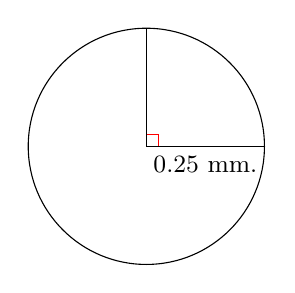
\begin{tikzpicture}[scale=0.75]
    \draw (0,0) circle [radius=2cm];
    \draw[red] (0,0) rectangle +(0.2,0.2);
    \draw (0,0) -- node [midway, below] {\small 0.25 mm.} (2,0);
    \draw (0,0) -- (90:2);
    \end{tikzpicture}
\end{enumerate}	\setcounter{Review}{\value{enumi}}

A belt runs on a pulley with radius 4 inches at 250 revolutions per minute.
\begin{enumerate} \setcounter{enumi}{\value{Review}}
\item Find the angular velocity in rad/sec. Round your answer to 2 decimal places.
    \item Find the linear velocity in ft/sec. Round your answer to 2 decimal places.
\end{enumerate}	\setcounter{Review}{\value{enumi}}

\newpage

\textsc{Angles and Radian Measure Key}

\begin{enumerate}
	\item $\frac{5\pi}{4}$  \newline\\
    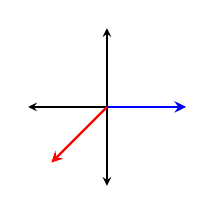
\begin{tikzpicture}
    \draw [<->, >=stealth](-1,0) -- (1,0);
    \draw[<->, >=stealth](0,-1) -- (0,1);
    \draw[->, thick, >=stealth, blue](0,0)--(1,0);
    \draw[->, thick, >=stealth, color=red](0,0) -- (-135:1);
    \bigangle[violet,thick]{-135}    
    \end{tikzpicture}
    
    \item $180^\circ$   \newline\\
    \begin{tikzpicture}
    \draw [<->, >=stealth](-1,0) -- (1,0);
    \draw[<->, >=stealth](0,-1) -- (0,1);
    \draw[->, thick, >=stealth, blue](0,0)--(1,0);
    \draw[->, thick, >=stealth, color=red](0,0) -- (180:1);
    \bigangle[violet,thick]{900}    
    \end{tikzpicture}
    
    \item $\frac{7\pi}{10}$ \newline\\
    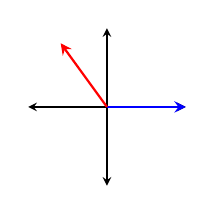
\begin{tikzpicture}
    \draw [<->, >=stealth](-1,0) -- (1,0);
    \draw[<->, >=stealth](0,-1) -- (0,1);
    \draw[->, thick, >=stealth, blue](0,0)--(1,0);
    \draw[->, thick, >=stealth, color=red](0,0) -- (486:1);
    \bigangle[violet,thick]{486}    
    \end{tikzpicture}
    
    \item $235^\circ$   \newline\\
    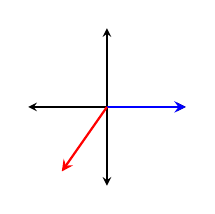
\begin{tikzpicture}
    \draw [<->, >=stealth](-1,0) -- (1,0);
    \draw[<->, >=stealth](0,-1) -- (0,1);
    \draw[->, thick, >=stealth, blue](0,0)--(1,0);
    \draw[->, thick, >=stealth, color=red](0,0) -- (-125:1);
    \bigangle[violet,thick]{-125}    
    \end{tikzpicture}
    
    \item $s = \frac{10\pi}{3}\,\mathrm{ft.}; \quad A = \frac{40\pi}{3}\,\mathrm{sq. ft.}$
    \item $s = \frac{26\pi}{9}\,\mathrm{cm.}; \quad A = \frac{52\pi}{9}\,\mathrm{sq. cm.}$
    \item $s = \frac{\pi}{8}\,\mathrm{mm.}; \quad A = \frac{\pi}{64}\,\mathrm{sq. mm.}$
    
    \item 26.18 rad/sec
    \item 8.73 ft/sec
\end{enumerate}